\documentclass[11pt]{article}
\usepackage{zed-csp,graphicx,color}%from
\pagenumbering{arabic}
\usepackage{geometry}
\usepackage{array}
\newcolumntype{L}{>{\centering\arraybackslash}m{3cm}}
\geometry{
	a4paper,
	total={170mm,257mm},
	left=20mm,
	top=20mm,
}
\begin{document}

\begin{titlepage}
\begin{figure}[h]
  \centerline{\small MAKERERE 
  
\includegraphics[width=0.1\textwidth]  {muk} UNIVERSITY}
\end{figure}
\begin{center}
	
	COLLEGE OF COMPUTING AND INFORMATION SCIENCES\\
	SCHOOL OF COMPUTING AND INFORMATICS TECHNOLOGY\\
	A REPORT ON\\
	FIELD ATTACHMENT/ INTERNSHIP AT\\
	(Name of Place of Attachment)\\
	Field Attachment Period (June 24th - August 06th .................)\\
	BY\\
	MUGUME IAN\\
	18/U/25478/PS\\
	Field attachment Report submitted to the School of computing and Informatics Technology\\
	In Partial fulfilment of the requirements for the degree of (state your Programme) of Makerere\\
	University Kampala\\
	
	MUGUME IAN \& ......................................\\
	
	
	Name \& Sign of Academic Supervisor .......................................................................\\
	(Date)\\
	Name \& Sign of Field Supervisor ........................................................................\\
	(Stamp \& Date)\\
\end{center}
\end{titlepage}

\newpage
\begin{center}
	\textbf{Declaration.}\\
	 I MUGUME IAN hereby declare that the information in this report is my own original
	 gathered authentic work. It also makes practical and effective fulfilment of the purposes and
	 objectives of this field attachment, and the content of the document has never been previously
	 submitted to any other university or institution for a higher degree or any other award. Except for
	 Citations, Quotations and References to other people’s work used where otherwise acknowledged.\\
	 
	 Date 4th August 2021\\
	 Signature…………………………………….\\
	\thispagestyle{empty}
\end{center}

\newpage

	\textbf{Acknowledgement.}\\
	First and foremost, I would like to acknowledge the Almighty God for the successful completion
	of the Field Attachment period.\\
	
	I would like to say thanks to Makerere University Data Science and Artificial Intelligence Lab for the opportunity given to me as
	an intern.\\
	
	Special thanks go to my academic supervisor Dr. Joyce Nabende for giving me an opportunity to work under the Data Science and Artificial Intelligence Lab, Makerere University.\\
	
	Many thanks to my field supervisor Mr. Tusubira Jeremy for his personal
	efforts, practical skills, professional guidance and direction towards successful internship.\\
	
	Finally, I would like to extend my heartfelt gratitude to my family members especially my mother
	RUTH KOMWAKA for all the support, classmates and other friends for their invaluable support
	throughout my training.\\
	\thispagestyle{empty}


\newpage

	\textbf{Abstract.}\\
	I carried out my Internship virtually under the Data Science and Artificial Intelligence with close supervision by both of my field and academic supervisors.\\
	
	One of the main aims of Bachelor of Science in Computer Science at undergraduate level is to solve real world problems around us for people and with this I was able to work on Diabetes disease prediction project using machine learning techniques being implemented with a Streamlit web application. I used two datasets from Kaggle website to work on my project and carried on tasks like EDA, data preprocessing, model formulation, building and evaluation, improving on their accuracies, saving the trained model using pickle library and then developing the streamlit web application basing on the two datasets for prediction.\\
	
	Throughout my work and experience, i attained problem thinking and solving skills, i was also able to troubleshoot some of the tasks which failed to output the required results through online research for solutions.\\
	
	The challenges faced include: hardships understanding new technical terms regarding machine learning, learning streamlit framework, poor internet connection, insufficient funds to buy mobile data bundles to continue with research and project.\\
	
	In my conclusion, internship under the Data science and AI lab was so productive with practical hands on skills and guidance from the experts like my field supervisor.\\
	
	I therefore recommend that we as students need to be taught much more of practical skills than theory and be given more time for practice.\\
	
	
	
	
	
	\thispagestyle{empty}


\newpage
\tableofcontents
\thispagestyle{empty}
\cleardoublepage
\setcounter{page}{1}

\newpage
\section*{List of figures.}
List of figures all in the Appendix section.\\

\newpage
\section*{List of tables.}
Figure 3.4 ..............................................................................................................................................26\\


\newpage
\section*{List of acronyms/abbreviations.}
EDA Exploratory Data Analysis.\\
PID	Pima Indians Dataset.\\
AI Artificial Intelligence.\\
NLP Natural language processing.\\
CSC Computer Science.\\
CoCIS College of Computing and Information Sciences.\\
FAMS Field Attachment Management System.\\

\newpage
\section{Introduction}\label{sec:intro}
\subsection{Introduction.}
This field attachment report is about the skills attained, lessons learnt, challenges, relatedness of
theory covered in class and recommendations during my internship placement at  Makerere University Data Science and Artificial Intelligence Lab from 24th June to 6th August 2021 . The report also
represents my experiences, recommendations and benefits of the field attachment[5].
\subsection{Background of the field attachment.}
Field attachment is a field-based practical training experience that prepares trainees for the tasks
they are expected to perform on completion of their programs. The main intention is to produce
practically oriented graduates that meet the required job-related competences of their future
employers
\subsection{Objectives of the field attachment.}
\begin{itemize}
	\item To enable students, get hands-on/real life experience they are expected to work in when
	they graduate.\\
	\item To provide an opportunity for students to apply the principles and techniques theoretically
	learnt into real-life problem solving situations. \\
	\item To provide an opportunity for students and academic staff to interact with the stakeholders
	and potential employers and thus appreciate field situations that will also generate
	information for curricula review and improvement.\\
	\item To develop student understanding of work ethics, employment demands, responsibilities
	and opportunities.\\
	\item To enhance and strengthen linkages between Makerere University and various
	stakeholders.\\
\end{itemize}

\subsection{Background of the organization of field attachment.}
The AI and Data Science research group is located at Makerere University's CoCIS Block B level 6 with office working hours starting at 9am to 6pm Monday to Saturday. Its being headed by Dr.Joyce Nabende who is also a lecturer. Its website is www.air.ug\\

The AI and Data Science research group at Makerere university specializes in the application of artificial intelligence and data science - including, for example, methods from machine learning, computer vision and predictive analysis- to problems in the developing world.\\

Applications: natural language processing for under-resourced languages, automated diagnosis of both crop and human diseases, auction design for mobile commodity markets, analysis of traffic patterns in African cities, and of telecoms and remote sensing data for anticipating the spread of infectious diseases.\\

VISION.\\
Excellence in Artificial Intelligence research for accessible solutions.\\

MISSION.\\
To advance artificial intelligence research to solve real-world challenges.\\

Objectives.\\
To apply Artificial intelligence research to African problems



\subsection{The structure of the organization.}
\begin{figure}[h]
	\centerline{\small 
		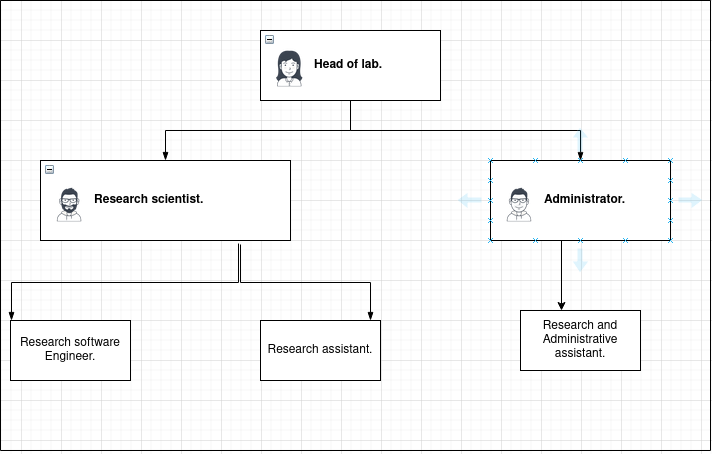
\includegraphics[height=0.4\textheight]  {chart}}
\end{figure}

\subsection{The main activities of the organization and ongoing IT projects.}
\begin{itemize}
	\item Organizing AI research seminars.\\
	\item Writing scientific research publication documents. \\
	\item Automated diagnosis of both crop and human diseases.\\
	\item Auction design for mobile commodity markets.\\
	\item Analysis of traffic patterns in African cities and of telecoms.\\
	\item Natural language processing (NLP) for under resourced languages.\\
	\item Remote sensing data for anticipating the spread of infectious diseases.\\
\end{itemize}

\newpage
\section{Student's Experiences.}\label{sec:intro}
\subsection{Title or Position occupied in an organisation.}
For the two months of the field attachment i under took virtually working on Diabetes Disease Prediction using a web application, I occupied the position of a full time Intern virtually with work schedule from Monday to Friday under the Makerere university Data Science and Artificial Intelligence lab. \\
\subsection{Duties and responsibilities.}
The following are the tasks I undertook during my field attachment and all were under supervision of my field supervisor;
\begin{itemize}
	\item General orientation via zoom meeting.\\
	\item Writing of concept paper.\\
	\item Getting and approving the two data-sets to use for my project.\\
	\item Exploratory Data analysis.\\
	\item Data pre-processing.\\
	\item Model selection and building.\\
	\item Improving on the accuracies of the models using Pipelines, Tuning and Ensembles.\\
	\item Model evaluation.\\
	\item Developing the web application.\\
	\item Presentation of the developed web application.\\
	\item Final report document writing.\\
	
\end{itemize}
\newpage

\subsubsection{Project walk though: Diabetes Disease Prediction using a web application/tool.}
I was able to do the project using two public datasets from Kaggle[1] ie Pima Indians dataset[2] and Early Diabetes disease prediction[3]. All source code was hosted on my Gihub repository[4].\\

\begin{center}
	\subsubsection*{Using Early Diabetes Disease dataset.}
\end{center}
\textbf{Phase 1: Exploratory Data Analysis.}
	\begin{itemize}
		\item There were 17 columns and 520 instances.\\
		\item There were no missing or null values.\\
		\item There were 320 positive cases for Diabetes and 200 negative cases.\\
		\begin{figure}[h]
			\centerline{\small 
				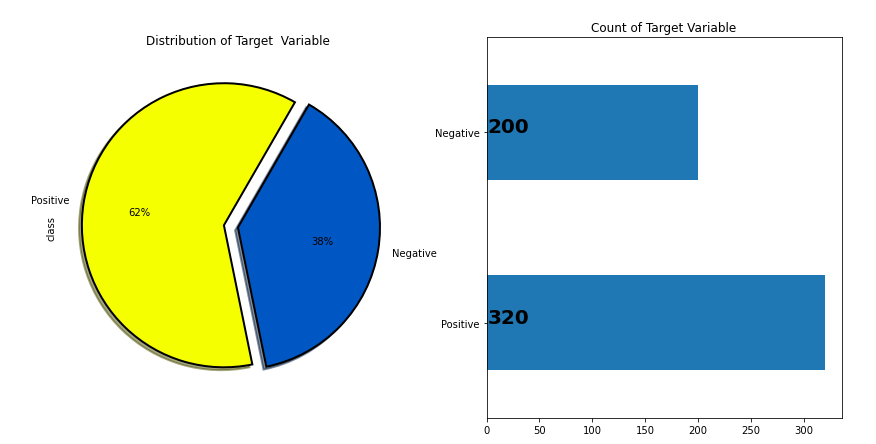
\includegraphics[height=0.3\textheight]  {pie}}
		\end{figure}
		
		\item The classes were randomly balanced between positive and negative cases though not much.\\
		\item Considering independent variables that have a high correlation with dependent variables and less correlation with other variables.\\
		\begin{figure}[h]
			\centerline{\small 
				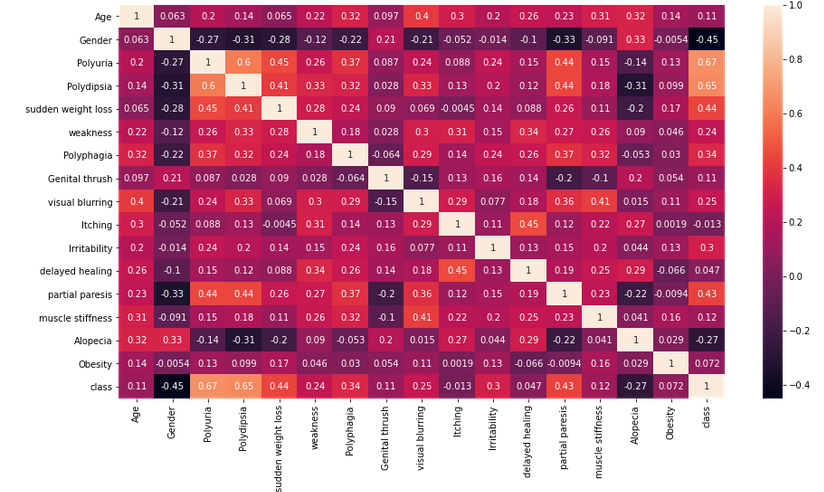
\includegraphics[height=0.2\textheight]  {corr}}
		\end{figure}
	
\newpage 
	
		\item Top 10 features.\\
		
			\begin{figure}[h]
				\centerline{\small 
					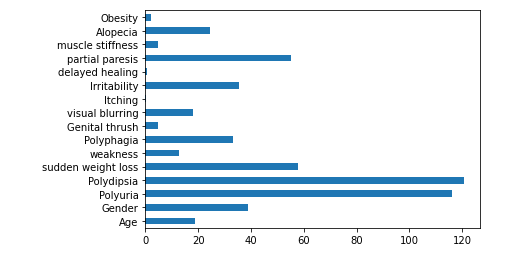
\includegraphics[height=0.3\textheight]  {top}}
			\end{figure}
		
	
		
	\end{itemize}

\textbf{Phase 2: Data preprocessing.}
\begin{itemize}
	\item For the 'Class' column (target variable) I converted positive and negative instances to binary values of 1 and 0 respectively.\\
	\item For the other columns with 'Yes'and 'No' instances, i used label encoder for object to numeric conversion.\\
	\item For the 'Age' column, i transformed those values to binary usin OneHOTEncoder.\\
	\item Finally all the instances in the column where in binary values.\\
	
	
\end{itemize}

\textbf{Phase 3: Model building, Improving performance accuracies and model evaluation.}
\begin{itemize}
	\item I chose 5 models for this classification problem eg SVM, Random forest classifier, Logistic regression and Naive Bayes.\\
	\item I used 10-fold cross validation with the 'accuracy' metric to get mean and standard deviation accuracies.\\
	\item I selected the 2 best models using the Box and whisker plots.\\
\newpage
	\begin{figure}[h]
		\centerline{\small 
			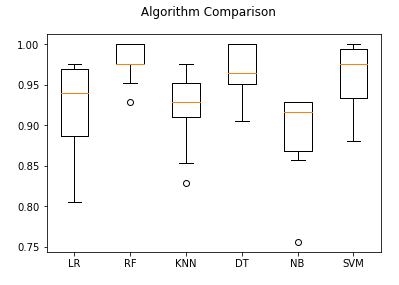
\includegraphics[height=0.2\textheight]  {box1}}
	\end{figure}
	
	\item For avoiding data leakage, i used Pipelines that standardised the data and build the model for each fold in the cross validation test harness.\\
	\begin{figure}[h]
		\centerline{\small 
			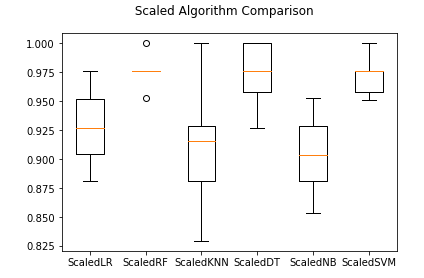
\includegraphics[height=0.2\textheight]  {box2}}
	\end{figure}
	From this figure of rescaled model using pipelines, 2 models were selected using Box and whisker plots, these were  Random Forests and Decision trees.\\
	
	\item Tuning Random Forests and Decision trees gave same accuracies of 98.0720.\\
	
	\item After using Ensemble methods, Extra Tree Classifier gave the better result.\\
	
	\item Drawing the Box and Whisker plots for the Ensemble methods, Extra tress classifier still showed better results again.\\
	
	\begin{figure}[h]
		\centerline{\small 
			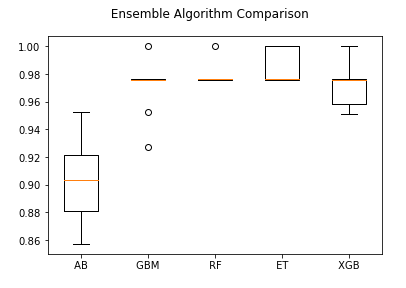
\includegraphics[height=0.2\textheight]  {box3}}
	\end{figure}
	
	
	
\end{itemize}

\newpage
\textbf{Phase 4: Finalising the model.}
\begin{itemize}
	\item I selected my best model using the Box and whisker plots, confusion matrix, precision and F1 scores.\\
	Selection of the best model was among the 3 models ie Random forests, Decision tree and extra tree classifier.\\
	Extra Tree Classifier was the best.\\
	\begin{figure}[h]
		\centerline{\small 
			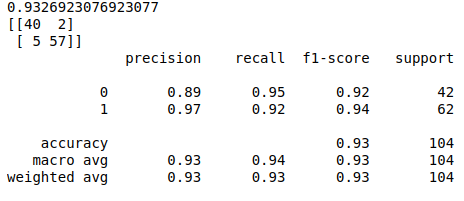
\includegraphics[height=0.2\textheight]  {res}}
	\end{figure}
	
	\item I later saved the pretrained model using pickle library.\\
	
	
	
\end{itemize}

\newpage
\begin{center}
	\subsubsection*{Using Pima Indians Diabetes dataset.}
\end{center}
\textbf{Phase 1: Exploratory Data Analysis.}
\begin{itemize}
	\item There were 9 columns and 768 instances.\\
	\item There were no data points missing in the dataset.\\
	\item There were some unexpected outliers in some columns after analyzing the histogram eg Blood pressure, age, insulin, BMI, glucose levels in reality can not be 0 since it doest make sense.\\
	\item The 'Outcome' column was the target variable for prediction. 1 was for positive case and 0 for negative case.\\
	\item In the 'Outcome' column, there was an imbalanced class distribution with 500 non diabetic and 268 diabetic people. The figure below shows the red part is for Diabetic, Blue is for the non-diabetic. For most of the attributes, the distribution for the diabetic people (the red part) is shifted towards the right when compared with the distribution of the non-diabetic part (blue part). This basically tells a story that a diabetic person is more likely to be a elder person with a higher BMI, SkinThickness, and glucose levels.\\
	\begin{figure}[h]
		\centerline{\small 
			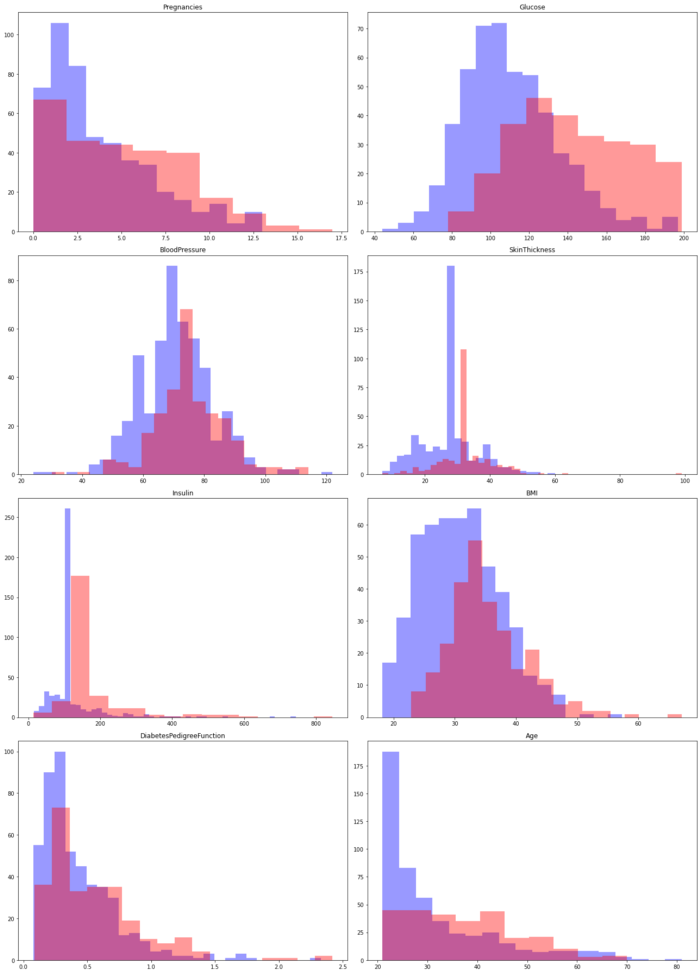
\includegraphics[height=0.5\textheight]  {hist1}}
	\end{figure}
	
	\item The classes were imbalanced between positive and negative cases.\\
	\begin{figure}[h]
		\centerline{\small 
			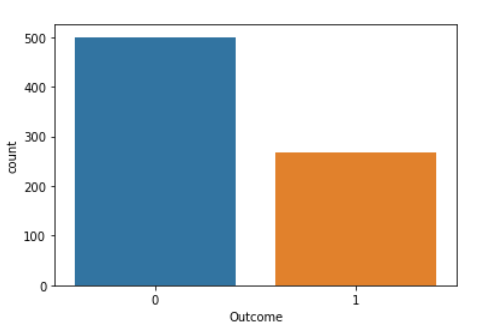
\includegraphics[height=0.3\textheight]  {p1}}
	\end{figure}
	
	\item plotting the boxplot for each of these attributes to clearly see the difference in the distribution of each of the attributes for both these outcomes (Diabetic and Non-diabetic)..\\
	\begin{figure}[h]
		\centerline{\small 
			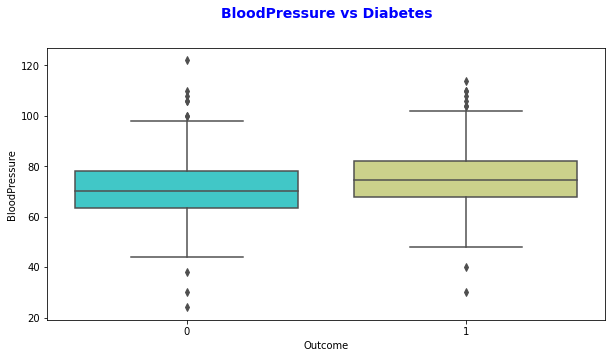
\includegraphics[height=0.2\textheight]  {bw}}
	\end{figure}
	\begin{figure}[h]
		\centerline{\small 
			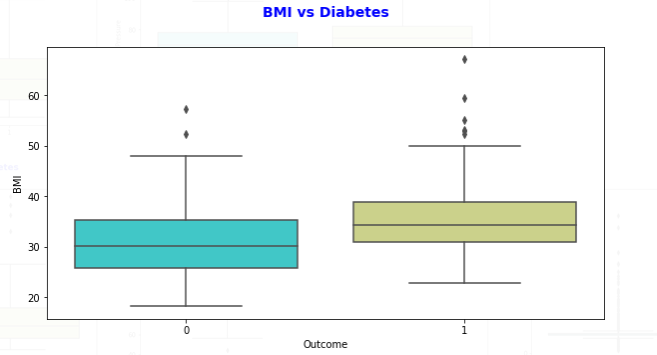
\includegraphics[height=0.2\textheight]  {bw2}}
	\end{figure}

	\begin{figure}[h]
		\centerline{\small 
			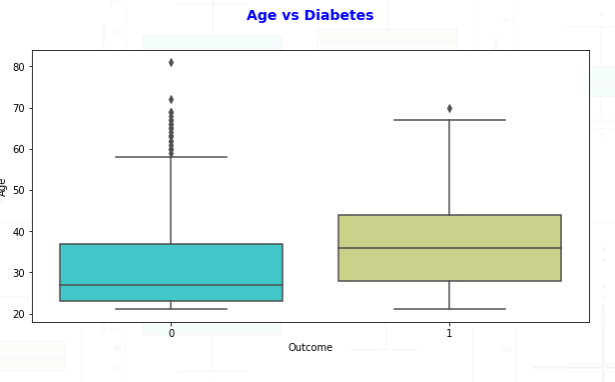
\includegraphics[height=0.2\textheight]  {bw3}}
	\end{figure}

	\begin{figure}[h]
		\centerline{\small 
			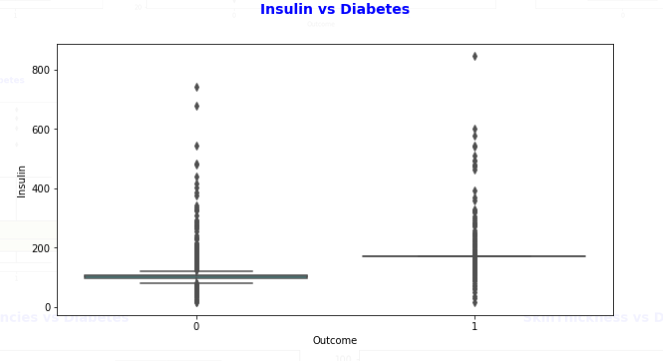
\includegraphics[height=0.2\textheight]  {bw4}}
	\end{figure}
\newpage
	\begin{figure}[h]
		\centerline{\small 
			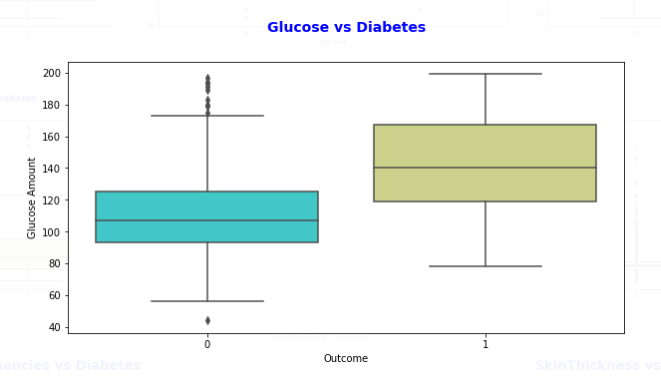
\includegraphics[height=0.2\textheight]  {bw5}}
	\end{figure}

	\begin{figure}[h]
		\centerline{\small 
			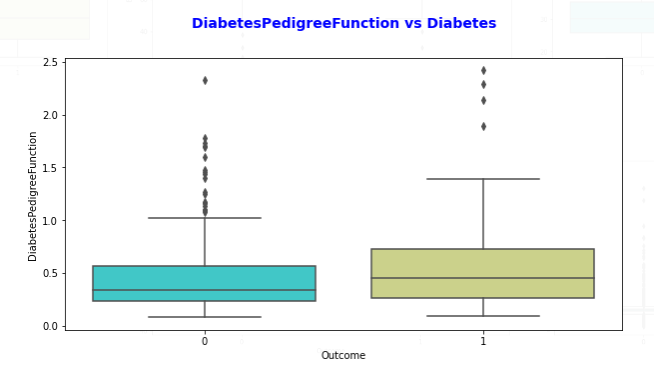
\includegraphics[height=0.2\textheight]  {bw7}}
	\end{figure}
	

	
	
	\newpage 
	

	
	
	
\end{itemize}

\textbf{Phase 2: Data preprocessing.}
\begin{itemize}
	\item For the unexpected outliers problem, i solved it by converting the zero values to null values and null values with imputation techniques like imputing using the median of that particular attribute based on what Outcome we will see. If a null value belongs to a diabetic person, next is finding the median using only the diabetic records, and similarly if it belongs to a non-diabetic person, finding the median using the non-diabetic records.\\
	\item All values in the dataset were put on the same scale using Standiser.\\
	
	
	
\end{itemize}

\textbf{Phase 3: Model building, Improving performance accuracies and model evaluation.}
\begin{itemize}
	\item I chose 5 models for this classification problem eg SVM, Random forest classifier, Logistic regression and Naive Bayes.\\
	\item I used 10-fold cross validation with the 'accuracy' metric to get mean and standard deviation accuracies.\\
	\item I selected the 2 best models using the Box and whisker plots ie Logistic regression and Random forests.\\
	\newpage
	\begin{figure}[h]
		\centerline{\small 
			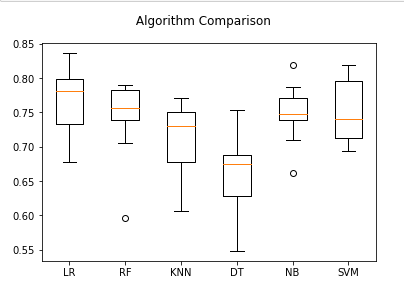
\includegraphics[height=0.2\textheight]  {y1}}
	\end{figure}
	
	\item For avoiding data leakage, i used Pipelines that standardised the data and build the model for each fold in the cross validation test harness.\\
	\begin{figure}[h]
		\centerline{\small 
			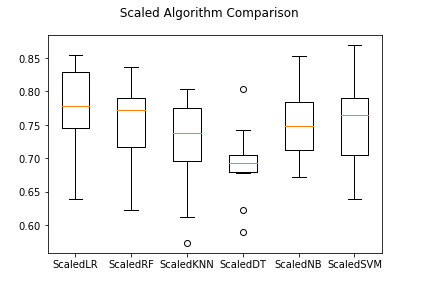
\includegraphics[height=0.2\textheight]  {y2}}
	\end{figure}
	From this figure of rescaled model using pipelines, 2 models were selected using Box and whisker plots, these were   Logistic model and SVM.\\
	
	\item Tuning Logistic regression and SVM gave same accuracies of Best: 0.775120 using {'C': 100, 'penalty': 'l2', 'solver': 'lbfgs'} and Best: 0.780090 using {'C': 0.1, 'kernel': 'linear'} respectively.\\
	
	\item After using Ensemble methods, Gradient boosting and Random forests both gave the better result.\\
	
	\item Drawing the Box and Whisker plots for the Ensemble methods, Random forests showed the best performance .\\
	
	\begin{figure}[h]
		\centerline{\small 
			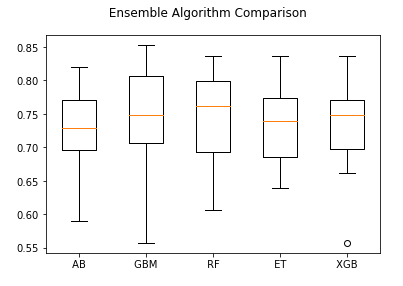
\includegraphics[height=0.2\textheight]  {y4}}
	\end{figure}
	
	
	
\end{itemize}

\newpage
\textbf{Phase 4: Finalising the model.}
\begin{itemize}
	\item I selected my best model using the Box and whisker plots, confusion matrix, precision and F1 scores on the 3 models ie SVM, Logistic regression and GBM..\\

	SVM was the best.\\
	\begin{figure}[h]
		\centerline{\small 
			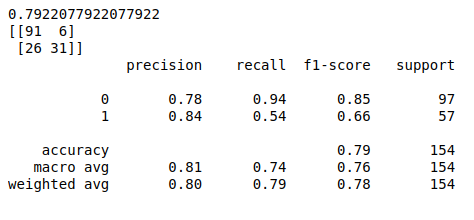
\includegraphics[height=0.2\textheight]  {y8}}
	\end{figure}
	
	\item I later saved the pretrained model using pickle library.\\
	
	
	
\end{itemize}




\newpage
\subsection{Supervision levels and relationship with Supervisor.}
\subsubsection{Supervision levels.}
My field supervisor was always available, provided corrective feedback, gave clear guidelines for
the application of theory, competent enough, and the supervisor provided support of the
professional development to me.
My field supervisor focused on competence with the accomplishment of meeting institutional
organization internship goals.\\

\subsubsection{Relationship with supervisor.}
There was a strong supervisory relationship with my field supervisor that effectively helped
successfully to participate in experiences and acquire competence.\\

Communication and feedback: My field supervisor always provided feedback to any asked question via email, and also commented on weekly progress reports.\\

Time management. My supervisor was very time conscious so I ensured that by every Wednesday per week i had completed weekly tasks and uploaded finished work to my Github repositry for him to evaluate on Thursdays. With this, my field supervisor gave time bound tasks to ensure proper good time management.

\subsection{Work Team and its composition - (by positions and not individual names).}
I majorly worked alone under close supervision and guidance of my field supervisor. For the case of machine learning concepts i wasn't clear about, i managed to watch tutorials, read research papers on ResearchGate website and also read text books to fully work on my project. All these improved onmy knowledge through research skills.


\newpage
\section{Evaluation on Field Attachment.}\label{sec:intro}
\subsection{Level of Accomplishment of duties and responsibilities assigned.}
To a greater extent I successfully accomplished the tasks assigned to me including corrections to my work.\\
Tasks included writing a concept paper, Doing EDA on both datasets, data preprocessing, model building and evaluation and also developing the web application using streamlit framework.



\subsection{New knowledge and skills gained in each of the duties and responsibilities.}
During field attachment I accumulated a lot of knowledge and skills. Each of the duties and
responsibilities as listed in section 2.2 empowered and greatly impacted on my skills.\\
\subsubsection{Knowledge.}
\begin{itemize}
	\item Machine learning.\\
	I was able to learn how to work with dataset csv files in for this like data preparation, EDA, data cleaning, data pre-processing, model building with cross validation and evaluation and also choosing the best model basing on metrics like precision, confusion matrix and recall.\\
	
	\item Web development.\\
	I was able to learn how to use Streamlit, an open source app framework for machine learning and data science teams for developing quick web interfaces with less code. 
	
	\item Research.\\
	I was able to accumulate lots of knowledge through research online like watching tutorials concerning machine learning, reading books and posts on machine learning blogs and also taking a Udemy course called Machine learning A-Z.
	
	\item Programming.\\
	I was able to improve on my knowledge in programming skills with python as i was using it in Jupyter notebook working environment.
	
	\item Version control.\\
	I was able to improve my skills using Github repository by using Git to keep track of all my source code files in their respective files.\\
	
\end{itemize}

\subsubsection{Skills.}
Computer competency, attention to detail, organization, problem solving, critical thinking, clear
written and spoken communication, time management, close listening.\\

\subsubsection{Responsibility.}
Working towards achieving my individual goals, Taking responsibility for my own professional and career development, Being open
and Accepting constructive feedback and take the initiative to improve, Giving feedback,
Completing any tasks and corrections assigned to me and applying the learning to improve my
performance , Keeping record of my performance achievements, successes and challenges i.e.
evaluation sheets downloaded from FAMS, Completing my self-appraisal by the specified deadline.


\subsection{Most interesting experiences.}
During the Field Attachment period, I really enjoyed the experience of working under Makerere University Data Science and Artificial Intelligence Lab  including
the comfortable working atmosphere, the technical guidance on the best Machine Learning practices and
the friendly relationship with both my field and academic supervisors. A list of interesting moments, are highlighted below.\\
\subsubsection{Internship project.}
Accomplishing my approved project on FAMS (Diabetes Disease Prediction using a web application). The
project involved several parts: Writing a concept paper, Exploratory Data Analysis on two data-sets, Data pre-processing, Model building, model evaluation, developing a responsive, attractive and interactive web application, report writing. It was a project which i did from scratch.\\
\subsubsection{Interaction with experienced people in the field.}
I had the opportunity to network with potential future employers and gain insight into the
types of employees they look for. Among them were my Field supervisor and a graduate friend of mine in the filed of machine learning. This made me realize the greatest value of Internship which is
providing a unique and exciting experience that is unparalleled in the classroom and to coordinate
job experience with academics.\\
\subsubsection{Learning IT area of interest.}
I really loved machine learning for its ability to make predictions based on some given data and of which most of predictions were usually right, that's what really excited me. 

\subsubsection{Working with experienced and more skilled individuals.}
I was able to work with my field supervisor who is experienced in this field of which i learnt skills like problem thinking and solving, trouble shooting some thing incase it failed to perform as expected in terms of python code and machine learning best practices to improve accuracy performance.


\subsection{Relatedness of University’s taught programmes to the Field of work.}
With the current curriculum for Undergraduate Bachelor of Computer Science program by NCHE,
Revised December 20, 2013 used by Makerere University. In its design goals which include
enabling students with computing and communication skills necessary for employment and career
opportunities in today’s ICT industries and business organization.\\

Illustration of relevance of computer science curriculum with to field work with few sampled
course units [6].\\

\begin{center}
	\begin{tabular}{ | m{20em} | m{20em}|  } 
		\hline
		COURSE UNIT & USE OF KNOWLEDGE FROM CLASS TO FIELD
		WORK  \\ 
		\hline
		BIS 1104: Communication skills for IT & Used for effective speaking and listening, meetings and
		presentation sessions  \\ 
		\hline
		CSC 2100: Data Structures and
		Algorithms & This enabled easy developing of problem solving
		systems.  \\ 
		\hline
		BSE 2105: Formal Methods & This enabled easy writing of stable and nice looking documents in Latex.  \\ 
		\hline
		CSC 3110: User Interface Design & This enabled developing interactive, responsive and attractive user interfaces..  \\ 
		\hline
		CSC 1100: Computer Literacy & I was able to learn skills of how to use the internet and also basic knowledge about computer organization .  \\ 
		\hline
		CSC 2114: Artificial intelligence & I learnt how to formulate and assess problems in AI. I also learnt how to implement software solutions to a wide variety of problems generally considered to require AI.  \\ 
		\hline
		BIT 2207: Research methodology & I learnt ethical research practices while writing documents. I also learnt various steps in the research process.  \\ 
		\hline
	\end{tabular}

Figure 3.4\\
\end{center}





\subsection{Challenges faced and how managed - (both work related \& organisational factors \& from an
	individual perspective).}
\begin{itemize}
	\item Limited time for the internship program is one of the challenges as it is only scheduled for
	eight weeks, which makes it not enough to learn experience most of all the activities
	undertook in a survey.\\
	
	\item Hardships understanding new technical terms regarding machine  learning. I managed to solve this through watching tutorials online, reading research papers on ResearchGate and also taking a course on Udemy.\\ 
	
	\item Delays in supervision to evaluate my work and make corrections were necessary by my field supervisor and also delays in filling up my progress reports on FAMS system. I managed to do this through continuous emailing and phone calling my field supervisor for continued assistance incase any.\\
	
	\item Poor internet connection and limited funds to buy mobile data bundles to keep up with research and work on my project. I managed to solve this by foregoing some of my luxuries to buy data bundles.\\
	
	\item Hardships developing the web tool for prediction using streamlit framework since it was new to me. I managed to solve this through watching tutorials online for help.\\
	

	
\end{itemize}


\subsection{Benefits derived from Field Attachment.}
The field attachment was of great importance, some of the benefits include;\\
\begin{itemize}
	\item Internship helped me understand work ethics, employment demands, responsibilities and
	opportunities.\\
	\item Field attachment provided career direction and confidence in my abilities by narrowing
	down the list of potential careers.\\
	\item My internship gave me the opportunity to try out Computer Science fields  i.e.
	machine learning and its applications in the world today.\\
	\item It prepared me for the working environment.\\
	\item It enhanced my CV needed to negotiate future jobs.\\
	
\end{itemize}

\subsection{Adequacy in University’s preparing the student for Field Attachment.}
In my view students having a limited range of skills in areas like communication and team work,
with educational experiences that can’t teach them how to solve problems with people whose
views are different than their own.\\

With less intercultural skills and an understanding of societies all this showed inadequacy of
preparation given to students for field attachment\\
\subsection{Preparedness of the Agency to receive and manage Students for Field Attachment.}
The Data science and AI lab shared some insight on the bigger picture and how their projects fit in internship goals
can bridge this knowledge gap. With the ability of College students having a lot to offer and will
approach things differently and the need to create a job description that is appealing, experience,
so it’s important to evaluate your needs and for both parties. This can be instrumental in targeting
younger clients and the clear setting of project goals and regular benchmarks to see how we interns
are performing clears shows lab was prepared. occasionally, resourceful persons and experts
in field always answered queries and also gave tips and shared experiences with the students. This
greatly inspired the me.

\subsection{Career Motivation.}
For the different values in regards to work and need for different things in the job market today
that include satisfaction and fulfillment. from the career motivation attained. This makes me plan
a more fulfilling and productive career and create an environment I can thrive in motivation's role
in influencing workplace behavior and performance at school.\\


\newpage
\section{Conclusions and Recommendations.}\label{sec:intro}
\subsection{Conclusions.}
Makerere university sends out students for field attachment with the main objective of enabling students to get hands on real life experiences in environments they are expected to work in after graduation. Although I did my internship virtually under the Data science and AI lab, it was well prepared to take on any student for field attachment since it had experts in the field to help and offer guidance to interns while carrying on their their projects.\\

I was exposed to new technologies in machine learning like Sci-kit learn, being able to work in Anaconda environment integrated with many tools like Jupyter lab and notebook, Visual studio code, Orange etc. I was able to use some of them to work on my project.\\

Summarized below are some of the strengths and weaknesses noted during internship in field attachment:\\
\textbf{Strengths}\\
The field attachment helped me to apply the knowledge taught at the university to the filed of work by working on real life projects eg Diabetes disease prediction using a web tool.\\  
My field supervisor was very helpful and offered great guidance while working on my project. This helped me learn alot of new knowledge and skills as indicated throughout this report.\\

\textbf{Weaknesses.}\\
On the side of the university, there was a weakness of late academic supervisor allocation that in turn delayed the supervision schedules.\\
The internship period set was in collision with semester work load on students.\\

\subsection{Recommendations.}
\subsubsection{Recommendations to the University.}
\begin{itemize}
	\item The university should urgently restructure the curricula offerings to meet the requirements
	of the labour market.\\
	\item This course CSC 2303: Field Attachment, should be shifted to the third year of study, such
	that it is given more time, at least six months. Many students have concluded that two
	months internships are too small.\\
	\item Students teaching-learning resources should be improved, especially the tools for
	practicals, lecture room capacity, laboratories and workshops.\\
	\item ICT should be introduced into both teaching and learning activities of every university, so
	that both staff and students can possess the much needed ICT knowledge and skills.\\
	\item The University should keep good records of its graduates for feedback purposes; while
	academic departments should liaise with employers for information on their employed ex-
	students.\\
	
\end{itemize}

\subsubsection{Recommendation to future interns.}
As students, good supervisory relationships are pivotal to successful completion of our degrees
because supervisors provide expert guidance in your research, and our fields of study thus need
for good supervisory relationships with our supervisors.\\

\newpage
\section{References and Appendices.}
\subsection{References.}
\begin{thebibliography}{100}  % 100 is a random guess of the total number of %references
	\bibitem{1} www.kaggle.com
	
	\bibitem{2}	https://www.kaggle.com/uciml/pima-indians-diabetes-database
	
	\bibitem{3}	https://www.kaggle.com/uciml/Early-diabetes-disease-database
	
	\bibitem{4} https://github.com/Group4Day2019/ML\_Internship2021
	
	\bibitem{5} Makerere University Council. (2011). Guidelines for Field Attachment. Retrieved June 5, 2016.
	from Makerere University Policies Website:
	http://policies.mak.ac.ug/sites/default/files/policies/GUIDELINES\_FOR\_FIELD\_ATTACHMEN
	T.pdf
	
	\bibitem{6} NCHE. (2013, December). Curriculum for Bachelor of Computer Science (CSC) Degree
	Program. Retrieved August 13, 2016, from https://courses.mak.ac.ug/programmes/bachelor-
	science-computer-science
\end{thebibliography}


\newpage
\subsection{Appendices.}
\subsubsection{Merged web tool with Pima Indians dataset selection.}
\begin{figure}[h]
	\centerline{\small 
		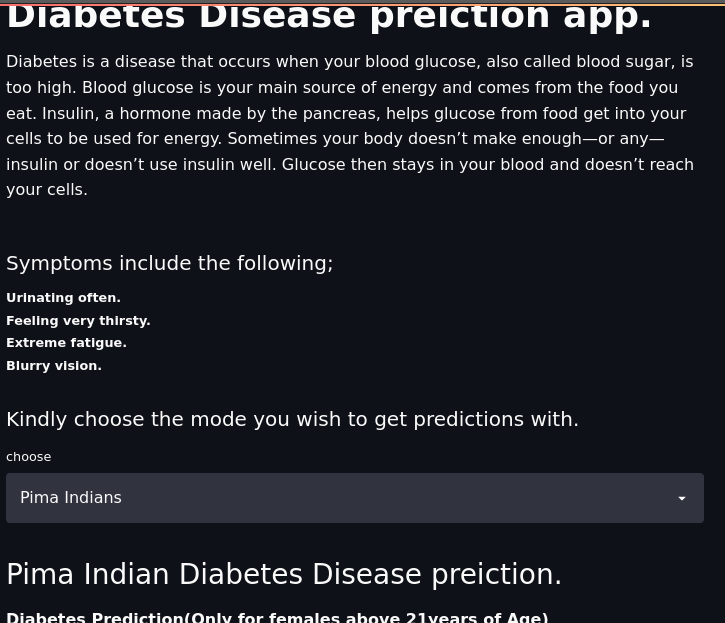
\includegraphics[height=0.4\textheight]  {Pmerged}}
\end{figure}

\subsubsection{Merged web tool with Early Diabetes Disease dataset selection.}
\begin{figure}[h]
	\centerline{\small 
		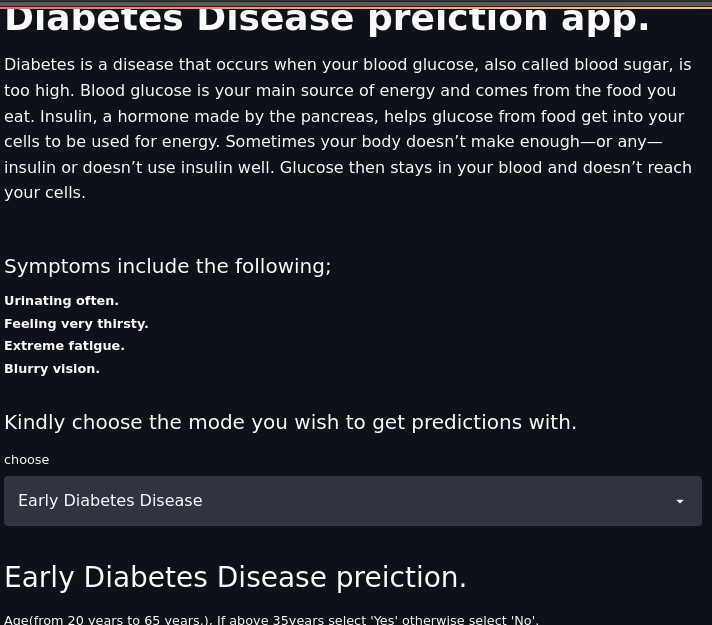
\includegraphics[height=0.3\textheight]  {Emerged}}
\end{figure}

\newpage
\subsubsection{Sample results of prediction on Pima Indians dataset regarding positive results.}
\begin{figure}[h]
	\centerline{\small 
		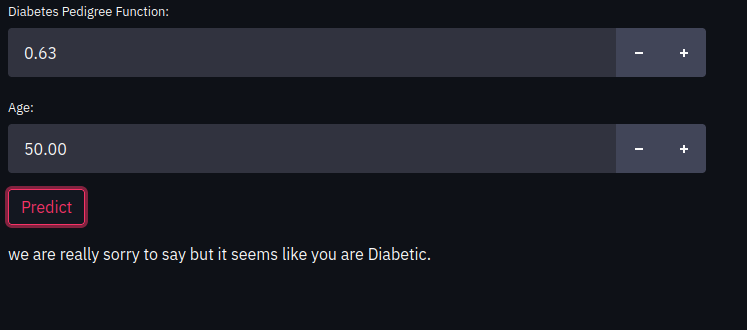
\includegraphics[height=0.25\textheight]  {Ppos}}
\end{figure}

\subsubsection{Sample results of prediction on Pima Indians dataset regarding negative results.}
\begin{figure}[h]
	\centerline{\small 
		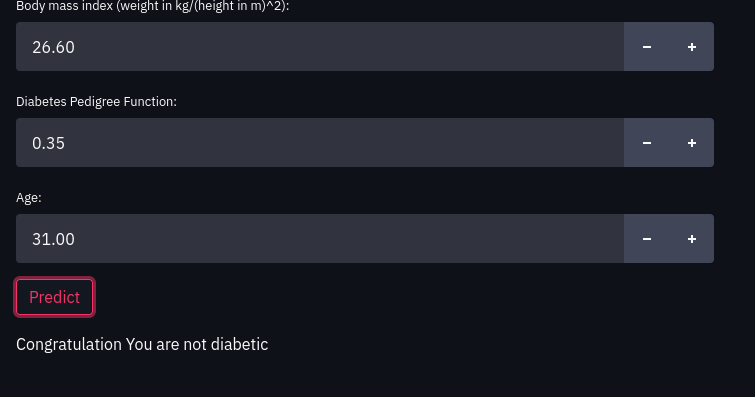
\includegraphics[height=0.25\textheight]  {Pneg}}
\end{figure}
\newpage
\subsubsection{Sample results of prediction on Early Diabetes Disease dataset regarding positive results.}
\begin{figure}[h]
	\centerline{\small 
		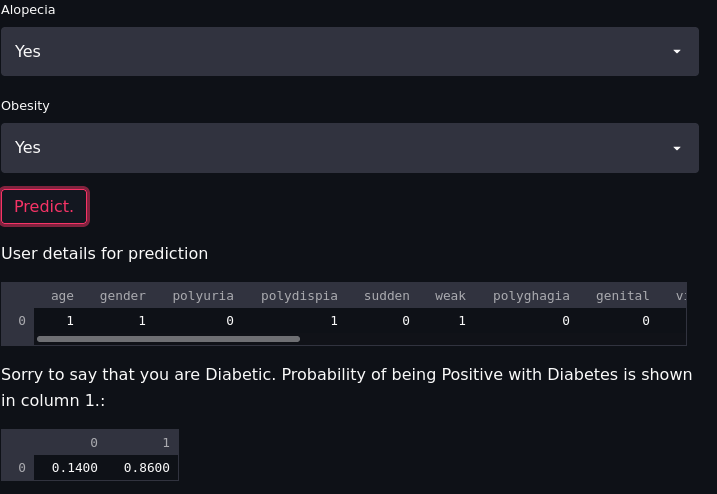
\includegraphics[height=0.35\textheight]  {Epos}}
\end{figure}

\subsubsection{Sample results of prediction on Early Diabetes Disease dataset regarding negative results.}
\begin{figure}[h]
	\centerline{\small 
		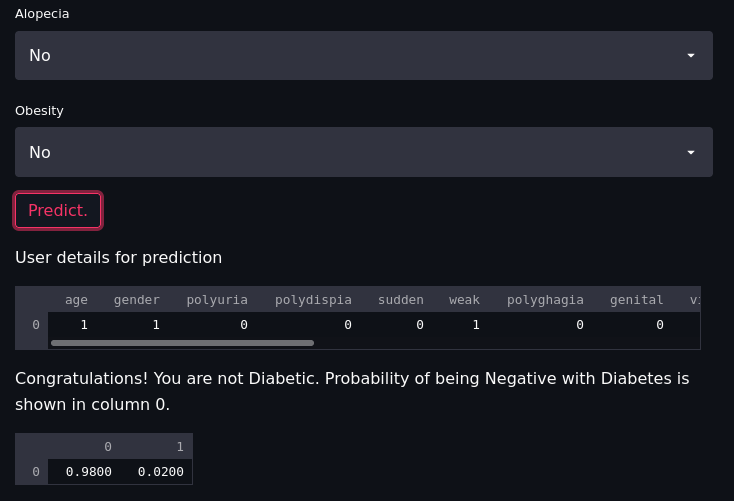
\includegraphics[height=0.35\textheight]  {Eneg}}
\end{figure}





\end{document}